% Draft figure environments for the manuscript (Figs. 2-10; Fig. 1, the block
% diagram fig:model, is drawn in TikZ by the integrator).
% Files: paper/figures/figNN_*.pdf, written by paper/figures/make_figures.py.
% Every figure is drawn at its final print size, the \textwidth of the elsarticle
% preprint (390 pt = 137.2 mm), so width=\textwidth includes it at 1:1 (text 7.5-8 pt).
% Every number quoted below is in paper/figures/figure_numbers.json, computed by
% make_figures.py from the arrays it plots; the % src: line after each caption
% names the stored files and the README section that state the same numbers.
% Needs: graphicx, siunitx (\SI, \si, \SIrange), amsmath, natbib.

\begin{figure}[!t]
\centering
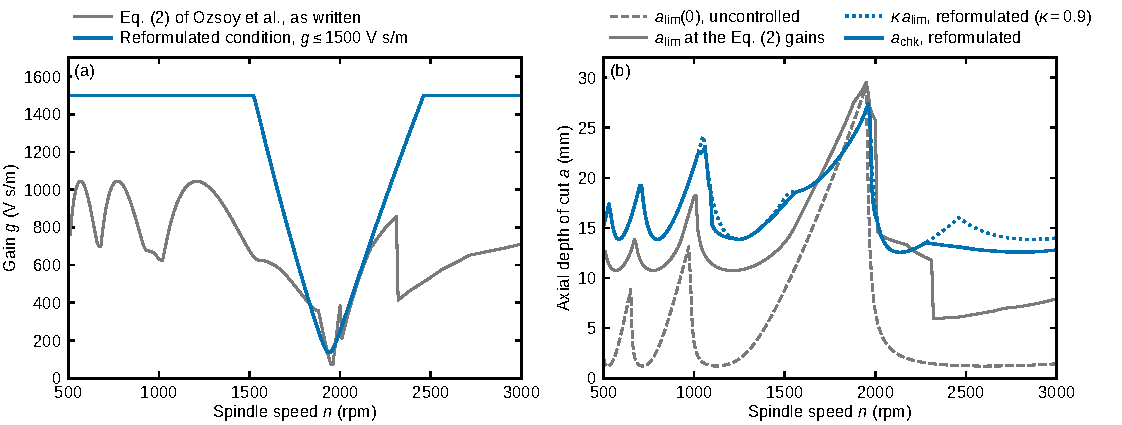
\includegraphics[width=\textwidth]{figures/fig02_feasibility.pdf}
\caption{Gain scheduling under the published feasibility condition and under the
reformulated authority condition (single identified mode, $\zeta=\SI{1.34}{\percent}$;
251 spindle speeds from \SI{500}{rpm} to \SI{3000}{rpm}). (a)~DVF gain $g$: the published condition of
\citet{ozsoy2026robust}, reproduced here with a step entry (the gain in
$[0,\SI{3000}{\volt\second\per\metre}]$ that maximises $a_{\lim}(g)$ while the peak force demand
$K_a g\lvert\dot x\rvert$ of a 50-revolution simulation from rest at $a_{\lim}(g)$ stays below
$F_{\max}=\SI{27}{\newton}$), and the
reformulated condition (steady forced command below \SI{9}{\volt} at every depth up to
$\kappa\,a_{\lim}$, $\kappa=0.9$, with $g\le\SI{1500}{\volt\second\per\metre}$), and the
published map of \citet{ozsoy2026robust} (verification/targets/fig8_gain_map.csv; dotted where it is a
straight line between optimised speeds: 500--550, 560--740 and 1410--\SI{1860}{rpm}).
(b)~Uncontrolled limit $a_{\lim}(0)$, linear limit $a_{\lim}$ at the gains of the published condition, and, at the
reformulated gains, $\kappa\,a_{\lim}$ and the checked depth
$a_{\mathrm{chk}}=\min(\kappa\,a_{\lim},\,a_{\mathrm{TD}})$, where $a_{\mathrm{TD}}$ is the limit
of a step entry from rest with the \SI{9}{\volt} clip in the time-domain simulator. The
reformulated gain sits on its bound at 157 of 251 speeds and falls to
\SI{134.9}{\volt\second\per\metre} at \SI{1940}{rpm}; $a_{\mathrm{TD}}$ governs
$a_{\mathrm{chk}}$ at 112 speeds. Mean depths: $a_{\mathrm{chk}}$ \SI{15.87}{\milli\metre}
(with the \SI{10}{\percent} margin), $a_{\lim}$ at the gains of the published condition \SI{12.75}{\milli\metre}
(without margin), $a_{\lim}(0)$ \SI{5.85}{\milli\metre}; the smallest $a_{\mathrm{chk}}$ is
\SI{12.57}{\milli\metre}, at \SI{2140}{rpm}.}
\label{fig:feas}
% src: results/feas_g1500.npz, results/feas_cert_g1500.npz, results/gainmap_main.npz, results/c1_map.npz; README sec. 8.2-8.4; figure_numbers.json (fig02)
\end{figure}

\begin{figure}[!t]
\centering
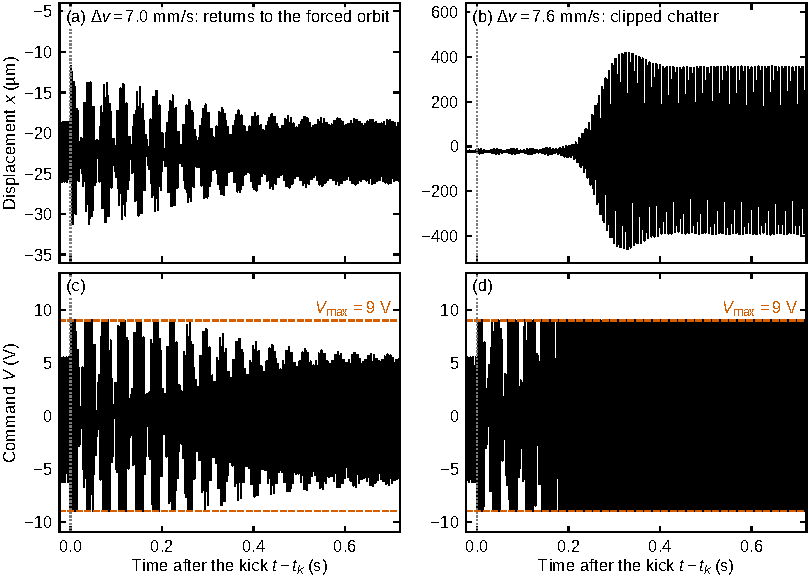
\includegraphics[width=\textwidth]{figures/fig03_two_outcomes.pdf}
\caption{The same linearly stable cut after a small and after a slightly larger kick:
\SI{2500}{rpm}, $g=\SI{1500}{\volt\second\per\metre}$, $a=0.9\,a_{\lim}=\SI{15.51}{\milli\metre}$
($a_{\lim}=\SI{17.24}{\milli\metre}$), $\lvert V\rvert\le\SI{9}{\volt}$,
$\zeta=\SI{1.34}{\percent}$, half-immersion down-milling, $f_z=\SI{0.05}{\milli\metre}$. The cut
is entered through the workpiece face, settles on the forced orbit, and the workpiece velocity is
kicked by $\Delta v$ at the start of revolution 100 (the first of 16 kick phases per tooth period);
time-domain simulation with the full surface memory. (a,~c)~$\Delta v=\SI{7.0}{\milli\metre\per\second}$:
displacement $x$ and command $V$ return to the forced orbit ($x$ between \SI{-26.0}{\micro\metre}
and \SI{-18.6}{\micro\metre}, $V$ between \SI{-6.2}{\volt} and \SI{5.5}{\volt}).
(b,~d)~$\Delta v=\SI{7.6}{\milli\metre\per\second}$: the motion grows into chatter with the command
clipped at $\pm\SI{9}{\volt}$ (dashed) and settles between about \SI{-390}{\micro\metre} and
\SI{360}{\micro\metre}. The stored critical kick at this phase is \SI{7.29}{\milli\metre\per\second}
(\SI{7.21}{\milli\metre\per\second} in the worst of the 16 phases).}
\label{fig:two}
% src: simulated by make_figures.py (fig03) with the protocol of src/c1_unsafe_zone.py (face entry, nreg 0, kick at revolution 100, 300-revolution classification); critical kicks: results/c1_basin.npz; README sec. 11.3, 11.5; figure_numbers.json (fig03)
\end{figure}

\begin{figure}[!t]
\centering
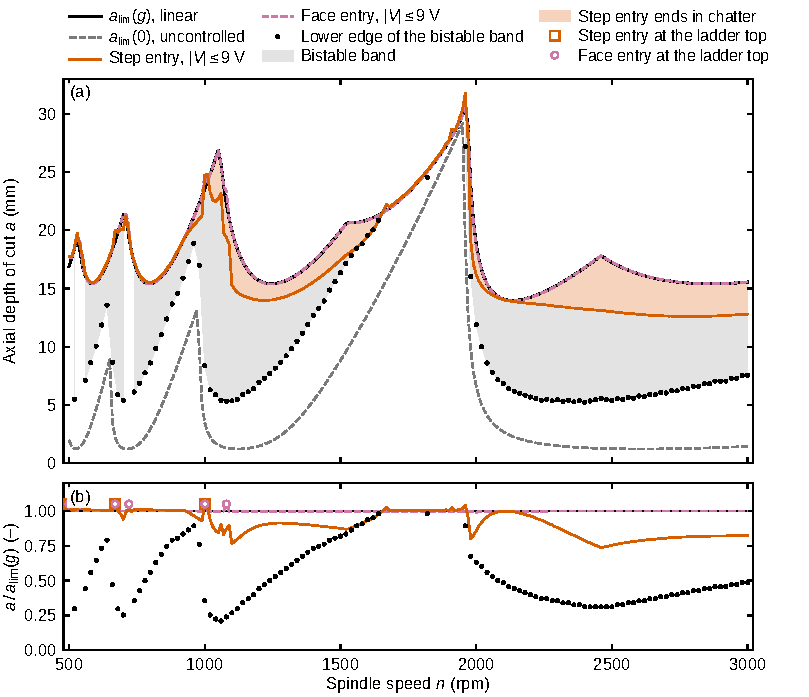
\includegraphics[width=\textwidth]{figures/fig04_entry_map.pdf}
\caption{Entry limits and the bistable band of the clipped DVF over 251 speeds, on the gain map of
the reformulated condition (Fig.~\ref{fig:feas}a; $\lvert V\rvert\le\SI{9}{\volt}$,
$\zeta=\SI{1.34}{\percent}$; time-domain simulation with the full surface memory, depths scanned
upwards in \SI{8}{\percent} steps from $0.25$ to $1.05\,a_{\lim}$, then bisected). (a)~Linear limit
$a_{\lim}(g)$ (zero-order approximation), uncontrolled limit $a_{\lim}(0)$, limits after a face entry
and after a step entry from rest, and the lower edge of the bistable band: every \SI{20}{rpm}, the
smallest depth at which one of seven kicks between \SI{3}{\milli\metre\per\second} and
\SI{3}{\metre\per\second}, at one of two phases, turns the settled cut into chatter (grey: from that
edge up to $a_{\lim}$; gaps: no band found, at 17 of 126 speeds). Light orange: depths at which the
step entry ends in chatter. (b)~The same limits divided by $a_{\lim}(g)$; open markers: step-entry
(squares, 4 speeds) and face-entry (circles, 6 speeds) limits at the top of the depth ladder,
$1.05\,a_{\lim}$, above which they were not resolved. The step-entry limit lies
below $0.97\,a_{\lim}$ at 157 of 251 speeds (median $0.91\,a_{\lim}$, minimum $0.736\,a_{\lim}$ at
\SI{2460}{rpm}); the face entry stays at or above $0.985\,a_{\lim}$; the band starts at
$0.21$--$0.98\,a_{\lim}$ (median $0.46$) and never below $1.08\,a_{\lim}(0)$. The 300-revolution
chatter classifier places simulated limits close to $a_{\lim}$ up to \SI{1.5}{\percent} high
(up to \SI{4.4}{\percent} near the forced resonance).}
\label{fig:map}
% src: results/c1_map.npz, results/c1_band.npz, results/c1_summary.json; README sec. 11.4, 11.7; verification/tdsim/check8_onset_long_runs.json, check10_forced_resonance_long_runs.json; figure_numbers.json (fig04)
\end{figure}

\begin{figure}[!t]
\centering
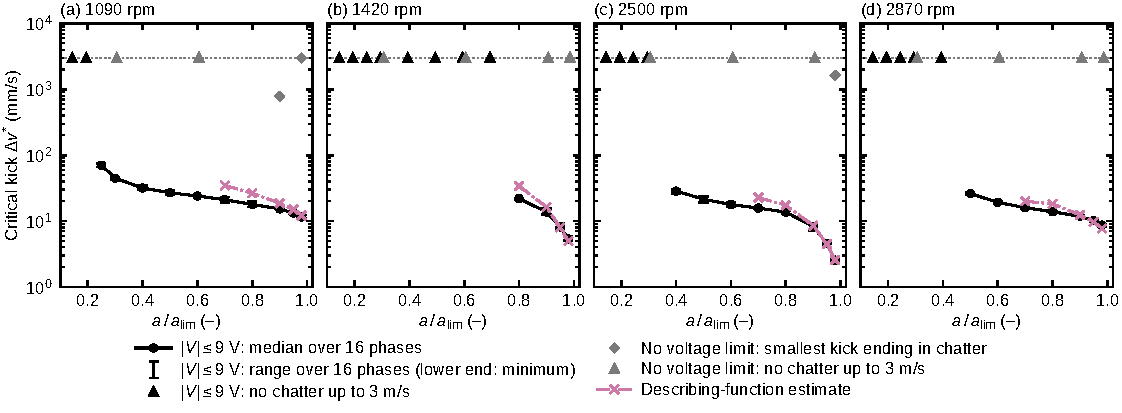
\includegraphics[width=\textwidth]{figures/fig05_basin.pdf}
\caption{Critical kick $\Delta v^*$ (the smallest velocity kick on the settled cut that ends in
chatter) against depth at the four basin speeds, $g=\SI{1500}{\volt\second\per\metre}$,
$\zeta=\SI{1.34}{\percent}$ (face entry, kick at revolution 100, outcome judged over the next 300
revolutions; kicks searched upwards on 16 sizes from \SI{0.1}{\milli\metre\per\second} to
\SI{3}{\metre\per\second}, then bisected to \SI{1.1}{\percent}). Black: with the \SI{9}{\volt} clip,
median (markers) and range (bars) over 16 kick phases per tooth period; the lower end of a bar is
the worst phase. Triangles on the dotted line at \SI{3}{\metre\per\second}: no chatter for any kick
up to this search limit (black: with the clip; grey: without a voltage limit). Grey diamonds:
without a voltage limit, the smallest kick that ends in chatter (one phase of 16). Purple: dual-input
describing-function estimate, converted to kick units with the chatter-mode factor of the linear
kicked cut (shown where that factor is fitted reliably). Right axis of (d): the kick as an equivalent displacement
$\Delta v^*/\omega_n$. At $0.98\,a_{\lim}$ the worst-phase critical
kick is \SIrange{2.34}{10.88}{\milli\metre\per\second}. Without the limit only 3 of the 16 tested
points chatter, after kicks of \SIrange{0.78}{3}{\metre\per\second}, so that there the clip shrinks
the basin 52 to 701 times. Simulated median over describing function: $0.61$--$1.13$; largest over
smallest critical kick across the phases: at most $1.24$.}
\label{fig:basin}
% src: results/c1_basin.npz, results/c1_df.npz, results/c1_summary.json; README sec. 11.5; figure_numbers.json (fig05)
\end{figure}

\begin{figure}[!t]
\centering
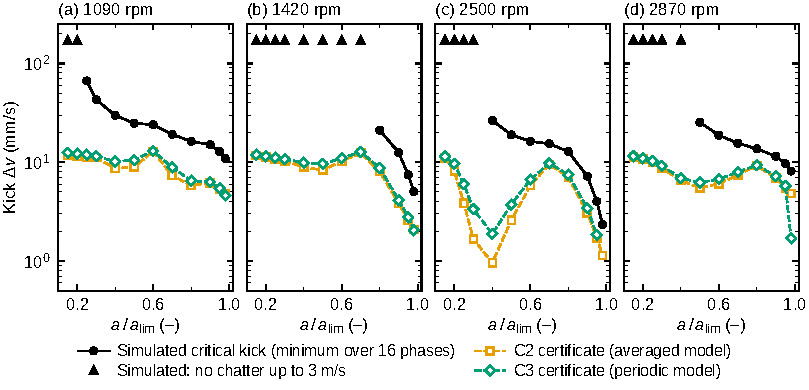
\includegraphics[width=\textwidth]{figures/fig06_certificates.pdf}
\caption{Certified kicks against the simulated critical kick at the 48 basin points of
Fig.~\ref{fig:basin} ($g=\SI{1500}{\volt\second\per\metre}$, $\lvert V\rvert\le\SI{9}{\volt}$,
$\zeta=\SI{1.34}{\percent}$). Filled: simulated critical kick, worst of 16 phases (triangles: no
chatter up to \SI{3}{\metre\per\second}). Open squares: C2 certificate, a sector-condition LMI on
the $N$-node collocation model of the averaged (zero-order) model, with the dead zone taken around
the forced command and the chip-validity bound $\lvert x-x(t-T)\rvert\le0.5f_z$. Open diamonds: C3
certificate on the time-periodic collocation model (periodic, piecewise-linear Lyapunov matrix on
16 subintervals of the tooth period). Both certify kicks in any phase and use the closed-form bound
of the forced command. C2 certifies all 48 points and lies below the simulated critical kick at all
29 points where one was found (ratio 1.48--27.6, median 2.34 from $0.7\,a_{\lim}$ up); C3 certifies
47 of 48 points (not \SI{2500}{rpm} at $0.98\,a_{\lim}$) and lies below the simulated kick at all 28
points (ratio 1.46--4.78 from $0.7\,a_{\lim}$ up, median 2.27); C3/C2 $=0.35$--$2.01$ (median
$1.064$). The certificates hold on the collocation models, not on the delay equation itself.}
\label{fig:cert}
% src: results/c2_validate.npz (rescaled as in src/c3_summary.py margin_errata), results/c3_basin.npz, results/c3_summary.json (basin, errata); README sec. 12.4, 14.5, 14.9; figure_numbers.json (fig06)
\end{figure}

\begin{figure}[!t]
\centering
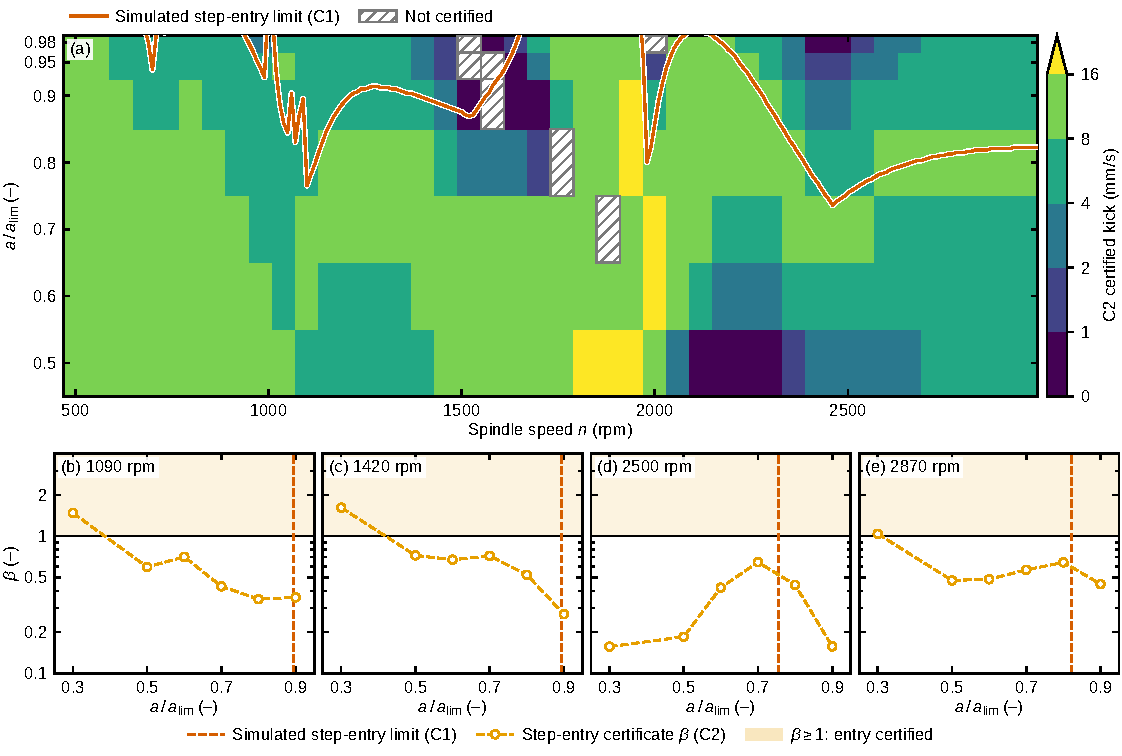
\includegraphics[width=\textwidth]{figures/fig07_certified_surface.pdf}
\caption{(a)~Certified kick of the averaged model (C2) over 42 speeds and the seven computed depths
0.5, 0.6, 0.7, 0.8, 0.9, 0.95 and $0.98\,a_{\lim}$, drawn as rows of equal height (not to scale in
$a/a_{\lim}$), on the gain map of the reformulated condition ($g\le\SI{1500}{\volt\second\per\metre}$,
$\lvert V\rvert\le\SI{9}{\volt}$, $\zeta=\SI{1.34}{\percent}$), in colour bins of a 1--2--5 sequence, with the
closed-form bound of the forced command; no certificate at 7 of 294 points, between \SI{1520}{rpm} and
\SI{2000}{rpm}: cross-hatched, the forced orbit itself reaches the clip ($u_0\le0$, three points);
hatched, no candidate passed the check ($u_0=0.04$--\SI{0.38}{\volt}, four points). Open circles: depths
above the simulated step-entry limit $a_{\mathrm{TD}}/a_{\lim}$ (Fig.~\ref{fig:map}b). At
$0.9\,a_{\lim}$ the certified kick is \SIrange{0}{16.0}{\milli\metre\per\second} (median
\SI{6.6}{\milli\metre\per\second}). (b--e)~Step-entry certificate $\beta$ against depth at the four
basin speeds: $\beta\ge1$ (shaded) certifies, on the averaged collocation model, that the cut entered
from rest on a fresh surface at tooth angle zero settles on the forced orbit; dashed: simulated
step-entry limit. $\beta\ge1$ only at $0.3\,a_{\lim}$ at \SI{1090}{rpm}, \SI{1420}{rpm} and
\SI{2870}{rpm} ($\beta=1.48$, $1.61$, $1.04$); at \SI{2500}{rpm} $\beta\le0.65$.}
\label{fig:surf}
% src: results/c2_surface.npz, results/c2_step.npz (both rescaled as in src/c3_summary.py margin_errata), results/c1_map.npz, results/c2_summary.json; README sec. 12.5, 12.6, 14.9; figure_numbers.json (fig07)
\end{figure}

\begin{figure}[!t]
\centering
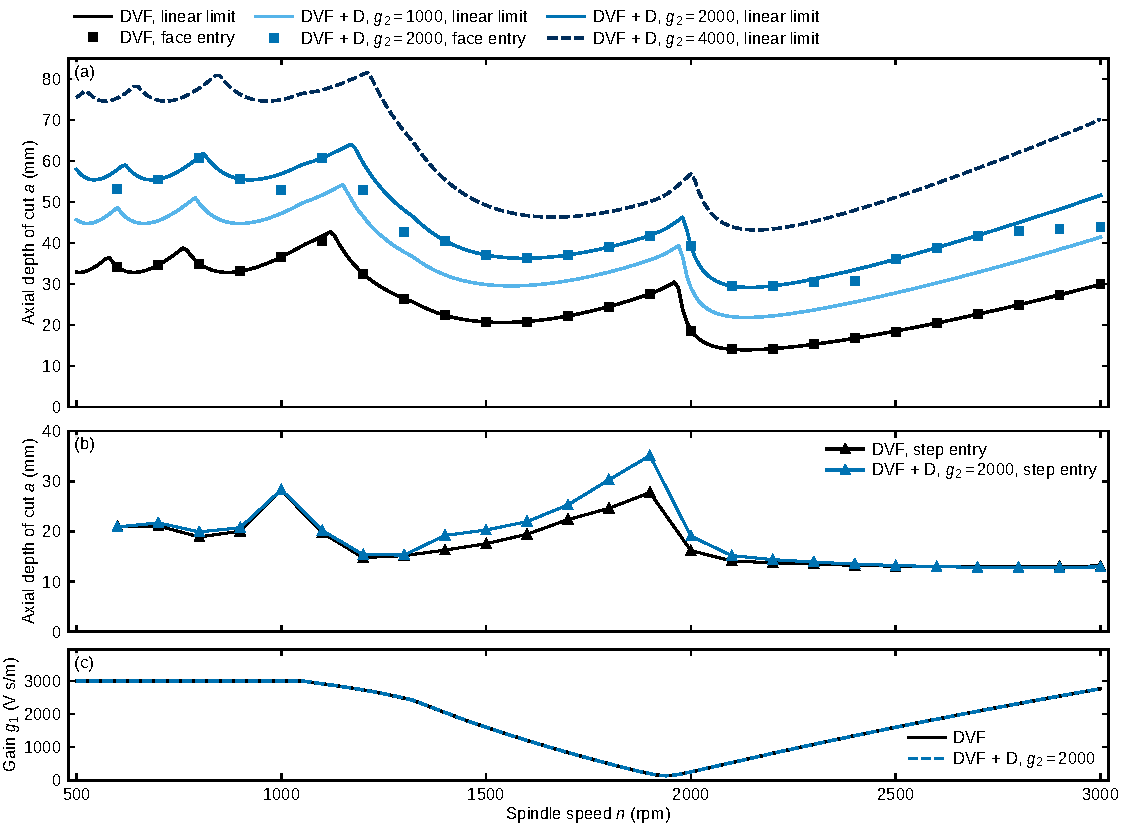
\includegraphics[width=\textwidth]{figures/fig08_delayed_limits.pdf}
\caption{Linear stability limit of DVF and of DVF with the delayed difference term (DVF\,+\,D) over
251 speeds under the same authority rule: the steady forced command stays below \SI{9}{\volt} at
every depth up to 0.9 of the design's own $a_{\lim}$, with $g_1\le\SI{3000}{\volt\second\per\metre}$
($\zeta=\SI{1.34}{\percent}$, zero-order approximation). (a)~Linear limits of DVF and of DVF\,+\,D
with $g_2=1000$, 2000 and \SI{4000}{\volt\second\per\metre}, and simulated limits after a face entry
with $\lvert V\rvert\le\SI{9}{\volt}$ (25 speeds) of DVF and of DVF\,+\,D with
$g_2=\SI{2000}{\volt\second\per\metre}$. Dash-dotted: $2D=\SI{32}{\milli\metre}$, twice the cutter diameter, exceeded by the linear limit at
71 (DVF) and 222 ($g_2=2000$) of 251 speeds. (b)~Simulated limits after a step entry from rest for the
same two designs. DVF is held below \SI{3000}{\volt\second\per\metre} by the
authority rule at 195 of 251 speeds, and adding $g_2$ hardly changes $g_1$ (not shown). With
$g_2=\SI{2000}{\volt\second\per\metre}$ the linear limit rises 1.44 to 2.10 times (median 1.78;
medians 1.43 for $g_2=1000$ and 2.40 for $g_2=\SI{4000}{\volt\second\per\metre}$), the face-entry
limit 1.45 to 2.12 times (median 1.72), the step-entry limit 0.98 to 1.27 times (median 1.03).}
\label{fig:dlim}
% src: results/c4_limits.npz, results/c4_entry.npz, results/c4_summary.json (limits, entry); README sec. 13.4-13.6; figure_numbers.json (fig08)
\end{figure}

\begin{figure}[!t]
\centering
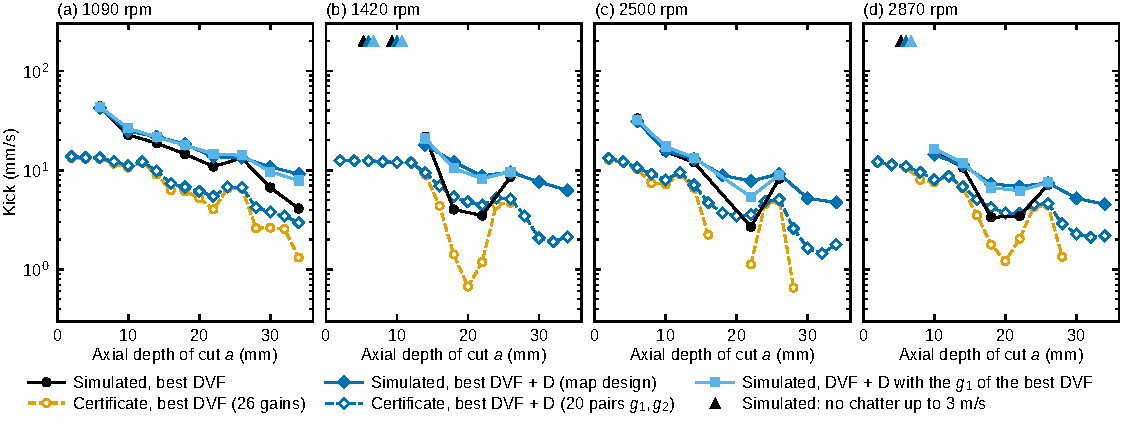
\includegraphics[width=\textwidth]{figures/fig09_delayed_basin.pdf}
\caption{Basin with the delayed term at the four basin speeds ($\lvert V\rvert\le\SI{9}{\volt}$,
$\zeta=\SI{1.34}{\percent}$). Open markers: certified kick on the averaged collocation model (the C2
inequalities with the delayed terms in the sector argument, closed-form bound of the forced command),
the best at each depth over 26 DVF gains ($g_1$ from 500 to \SI{3000}{\volt\second\per\metre}) and
over 20 delayed pairs ($g_1\in\{500,1000,1500,2000,3000\}$,
$g_2\in\{500,1000,2000,4000\}$\,\si{\volt\second\per\metre}); gaps: nothing certified. Filled
markers: simulated critical kick (worst of 16 phases) of the best DVF design, of the delayed design
of the gain map, and of the best DVF gain $g_1$ with $g_2=\SI{500}{\volt\second\per\metre}$ added
(the same forced command as that DVF); triangles: no chatter up to \SI{3}{\metre\per\second}. At the
100 simulated design points the certificate lies below the simulated critical kick wherever one was
found (89 of 89; ratio 1.60--7.32, median 2.29). Requiring a certified kick of at least
\SI{1}{\milli\metre\per\second}, every grid depth up to \SI{34}{\milli\metre} is certified with the
delayed term at all four speeds, against 16 to \SI{34}{\milli\metre} for the best DVF. With the
same forced command the simulated critical kick grows 1.79 to 2.59 times (median 2.00) at the six pairs where the DVF certificate is at most
\SI{2.1}{\milli\metre\per\second}, and 0.96 to 2.59 times (median 1.14; larger at 19 of 22 pairs)
over all pairs.}
\label{fig:dbasin}
% src: results/c4_gainmap.npz (rescaled as in src/c3_summary.py margin_errata), results/c4_validate.npz, results/c4_validate2.npz, results/c4_summary.json (validate2), results/c3_summary.json (errata c4_validate); README sec. 13.7, 13.8; figure_numbers.json (fig09)
\end{figure}

\begin{figure}[!t]
\centering
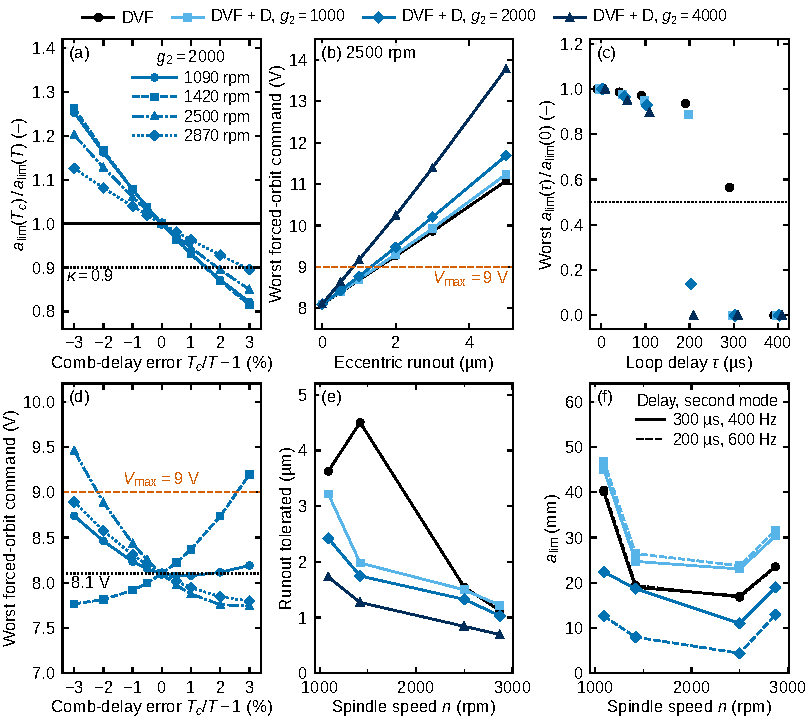
\includegraphics[width=\textwidth]{figures/fig10_robustness.pdf}
\caption{Robustness of the delayed term (closed-form zero-order model; each design takes the largest
$g_1\le\SI{3000}{\volt\second\per\metre}$ that keeps the forced command below \SI{8.1}{\volt}, a
\SI{10}{\percent} guard band, up to $0.9\,a_{\lim}$; $\zeta=\SI{1.34}{\percent}$). (a)~Linear limit
with a comb-delay error $T_c/T-1$, relative to the exact delay ($g_2=\SI{2000}{\volt\second\per\metre}$;
dotted: $\kappa=0.9$), and (d)~largest forced-orbit command over the design depths for the same
cases. (b)~Largest forced-orbit command at \SI{2500}{rpm} against an eccentric radial runout of the
teeth (worst of eight runout phases) and (e)~the runout at which it reaches \SI{9}{\volt}.
(c)~Loop delay $\tau$ with an assumed, not identified, second mode at \SI{400}{\hertz} or
\SI{600}{\hertz} ($k_2=6k$) or at \SI{800}{\hertz} ($k_2=40k$), $\zeta_2=\SI{1}{\percent}$:
$a_{\lim}(\tau)/a_{\lim}(0)$, worst over the four speeds and the three modes, at the computed delays
only (markers offset horizontally; 0: loop unstable without cutting); dotted: one half. (f)~$a_{\lim}$
at the four speeds with \SI{300}{\micro\second} and the \SI{400}{\hertz} mode (solid) and with
\SI{200}{\micro\second} and the \SI{600}{\hertz} mode (dashed). At $\pm\SI{2}{\percent}$ comb-delay
error the forced command stays within \SIrange{7.76}{8.89}{\volt}, but at $+\SI{2}{\percent}$ the
limit falls to 0.87--0.93 of its nominal value. The runout tolerated is
\SIrange{1.12}{4.50}{\micro\metre} for DVF, \SIrange{1.03}{2.42}{\micro\metre} for $g_2=2000$ and
\SIrange{0.69}{1.73}{\micro\metre} for $g_2=\SI{4000}{\volt\second\per\metre}$. The limit stays
above one half of its delay-free value up to \SI{300}{\micro\second} for DVF, \SI{200}{\micro\second}
for $g_2=1000$ and \SI{100}{\micro\second} for $g_2=2000$ and 4000.}
\label{fig:robust}
% src: results/c4_robust.npz, results/c4_summary.json (robust); README sec. 13.9, 13.10; figure_numbers.json (fig10)
\end{figure}
